
Одним из возможных путей разрешения являются графовые модели знаний, основанные 
на байесовых сетях. \footnote{Альтернативный подход заключается в обучение языковой модели работе с инструментами. Таковыми могут быть калькуляторы,
языки программирования или поисковые инструменты.} Такие сети представляют представляют связь между понятиями вероятностно, 
задавая причинно-следственный аппарат как направление в ребре связи графа. 
Итоговая модель представляет собой статистическую модель явления, которую можно использовать для
управления и анализа системой. 

Описанный подход называется \textit{вариационным причиннно-следственным выводом}. Направление развивается на стыке логики,
теории алгоритмов и графового анализа. Разработанные модели применяются в  
Автор видит большой потенциал в заданных моделях и 

\section{Предметный обзор направления исследования}

\subection{Введение}

Графовое представление позволяет разрешать мысленные парадоксы причинности.

\begin{figure}[h]
    \centering
    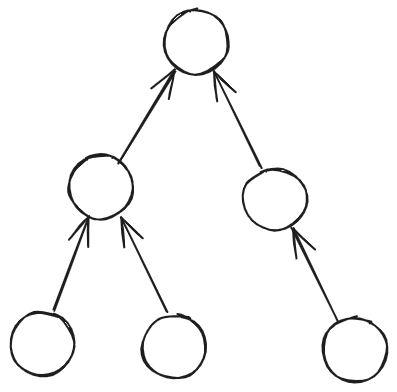
\includegraphics[width=0.5\textwidth]{assets/graph.excalidraw.png}
    \caption{Графовое представление}
    \label{graph}
\end{figure}





Таким образом, проведенный анализ позволяет судить о достоверности суждений и том, как именно их нужно изменить 
для получения более

Зададим ключевые предметные определения.

\subsection{Направление исследования} 


Формально опишем заданные в предисловия пожелания к аппарату вероятностных графовых моделей.


\begin{figure}[h]
    \centering
    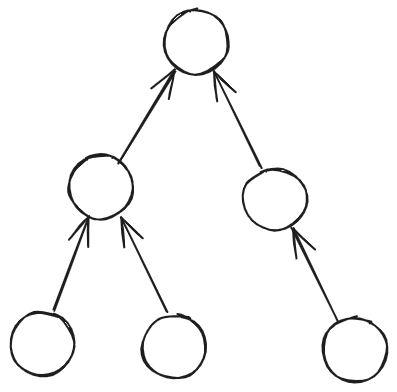
\includegraphics[width=0.5\textwidth]{assets/graph.excalidraw.png}
    \caption{Графовое представление}
    \label{graph}
\end{figure}

\subsection{Изучение причинно-следственные связи}



Таким образом порождающая дискриминативной модели являются возможность порождения.


\textit{Определение} Графовой вероятностная модель называется граф $\Gamma = (E,V)$, где для каждого 

Графовые модели принципиально различаются на марковские поля
\footnote{термин поля связан с определенными операциями сложения и ренормализации формально соотвествующим требованиям поля}
и байесовы сети \cite{lafferty2001conditional}.


\begin{figure}[h]
    \centering
    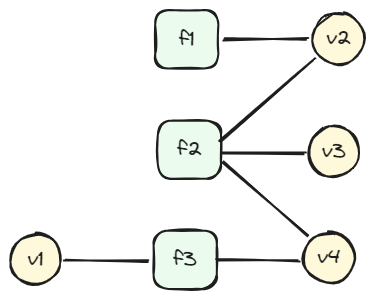
\includegraphics[width=0.5\textwidth]{assets/factor_graph.excalidraw.png}
    \caption{Фактор-граф представляет}
    \label{graph}
\end{figure}


\subsection{Выбор оптимальной модели}


Выбор топологии графа выполняется по принципу Оккаме: граф должен быть прост, но исчерпывающе описывать постановку. Для этого
все параметры модели согласно байесовскому подходу задаются случайными величинам с известными статистическими распределениями.М
После сравнивая маргниальную вероятность всех возможных форм граф находится наилучшая конфигурации $\Gamma$. Такой подход, в общем
случае требует значительных вычислительных ресурсов, поскольку маргинализация является NP-полной задачей, экспоненциально усложняющейся
с числом роста фактором.

Обновление представлений 

Алгоритмы выполняющий расчет


\subsection{Байесовы сети}

Для байесовых сетей 

\begin{figure}[h]
    \centering
    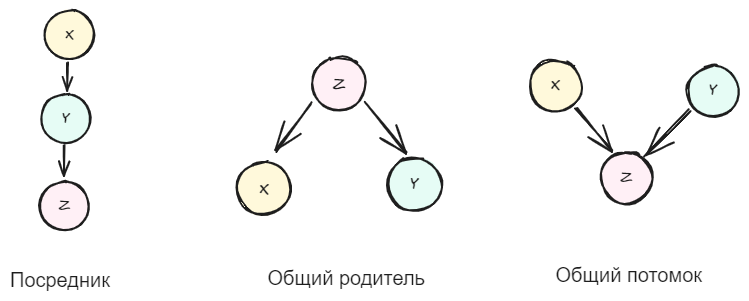
\includegraphics[width=0.5\textwidth]{assets/bayes_net.excalidraw.png}
    \caption{Элементарными структурами байесовых сетей являются группы }
    \label{bayes-net}
\end{figure}


\subsubsection{Вариационный причино-следственный анализ}

Ключевым для анализа полученного графа является понятие потока зависимостей, задающего связь между наблюдаемой и инструментальными переменными.
Задача специалиста найти способ на заданных данных свести многокомпонетный анализ, осложненный учетом
взаимного влияния факторов друг друга, к изучения влияния одного признака. Такая задача, как правило, выполняется через 
фиксации прочих признаков через зависимые. 

\textit{Определение} (от \texit{англ. cofounder} ) 


\textit{Определение} \textit{Интервенция} называется


\subsubsection{Техники}

Причинно-следственной связь

Оптимизация графовой модели выполняется посредством аггрегации сообщений соединненых ребер.

\begin{figure}[h]
    \centering
    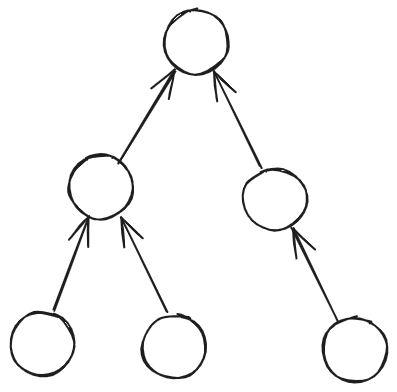
\includegraphics[width=0.5\textwidth]{assets/graph.excalidraw.png}
    \caption{Таксономия современных подходов обработки естественного языка}
    \label{llm_taxonomy}
\end{figure}



\section{Теоретический аппарат}




Аналитическое исследование причинно-следственных связей на данных выполняется с помощью генеративных графических моделей.

Для анализа используются маргни



Принципиально рассчитывается вероятность заданной цепочки логических рассуждения .
Опишем постановку более формально с введением и ключевых понятий и пояснением метода оптимизации. 

\textit{Определение} Вероятностная модель называется графовой, если ребра графа

Каждое ребро графа имеет вероятностную модель $P(X|A)$, в простейшем случае представленную ло

Таким образом, граф с наибольшей вероятностью является. 

\begin{equation}
    x^t_{i+1} = x_i + f(x_1, \dots, x_n), 
\end{equation}

$$
    \lambda_n  f(x_1, \dots, x_n), 
$$


\texit{Определение} Случай дерево

\section{Научно-образовательная деятельность автора}

\subsection{Изданные работы}



